\chapter{Results}\label{chap:results}


%Describe the experimental setup, the used datasets/parameters and the experimental results achieved

This section will give an overview over the used datasets, the used metric to evaluate our models, the configuration of our model and finally the experimental results achieved.

\section{Dataset}
In this implementation we mainly used the text8 \footnote{matt mahoney.zip} dataset. We chose this dataset for two reasons. First of all it's a very small dataset, more on exact specifics later, that enabled us to do a lot of computations. Secondly this data set was used in a lot of related work (cite gpu, cpu,) hence giving us a very good benchmark. The text8 dataset consists of 1702 lines of 1000 words, there is no punctuation. Know we had to choose between building arbitrary sentences and keeping the dataset as it is. We chose the first option because it gives us a faster computation time, and did not show any loss in accuracy empirically. We chose a sentences length of 20. Furtheremore we applied a technique called subsampling that reduces the data set size. 
We needed a second more larger dataset to confrim our results.  We therefore chose the enwik9 dataset\footnote{matt enwik9}. This datast neede some more preprocessing as it's plain html. We therefor used the script that can be found at the bottom of this page\footnote{script}. We applied exactly the same preprocessing technique afterwards.
We will know explain the technique called subsampling. 


 
 
 
\subsection{Subsampling}
Subsampling is a technique introduced by Mikolov et al. in \cite{mikolov} to reduce the dataset size while at the same time increasing the quality of the dataset, i.e getting better word embeddings. Certain words that appear very frequently in the dataset such as: "the, as, it, of" do not give an intrinsic value to the words that appear in it's context. Therefore the idea of subsampling is to delete such words from the dataset. This will decrease the computation time and should in theory increase the accuracy of the model. The increase in accuracy can also be explained by the fact that words that would not have appeared in the context of each other, may know, because words between have been deleted, do.
Know the question arises, how one chooses to delete a word. Mikolov et al. chose the following equation to compute the deletion of a word $w$ in the data set:
\begin{equation}
P(w) = 1- \sqrt{{\frac{t}{f(w)}}}
\end{equation}
where $f(w)$ is the frequency of w, and $t$ is a threshold set empirically. (Mikolov et al.)  recommends a value between $0$ and $10^{-5}$, depending on the size of the dataset. We experimented with different values and $10^{-4}$, seemed the most suited. We did this by simply looking at a random set of sentences and humanly judging the results. Stats about subsampling can be found in table \ref{table:treshold}. Examples in figure \ref{fig:treshold_examples}

\begin{table}[h]
\centering
\begin{tabular}{|l|l|l|l|l|l|}
\hline
Sampling Treshhold &  0      &      $ 1^{-1}$&$   1^{-2}$& $1^{-3}     $ &$1^{-4}   $    \\ \hline
Size of Dataset    & 16 mio & 15mio & 11 mio & 8mio & 4 mio \\ \hline
\end{tabular}
\caption{Size of preproccessed text8 dataset according to sampling treshold}
\label{table:treshold}
\end{table}

\begin{figure}
    \centering
    \begin{subfigure}[b]{\textwidth}
        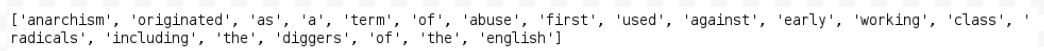
\includegraphics[width=\textwidth]{treshold1}
        \caption{Treshold = $10^{-1}$}
        \label{fig:treshold1}
    \end{subfigure}
    ~ %add desired spacing between images, e. g. ~, \quad, \qquad, \hfill etc. 
      %(or a blank line to force the subfigure onto a new line)
    \begin{subfigure}[b]{\textwidth}
        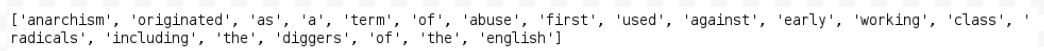
\includegraphics[width=\textwidth]{treshold1}
        \caption{Treshold = $10^{-2}$}
        \label{fig:treshold2}
    \end{subfigure}
    ~ %add desired spacing between images, e. g. ~, \quad, \qquad, \hfill etc. 
    %(or a blank line to force the subfigure onto a new line)
     \begin{subfigure}[b]{\textwidth}
        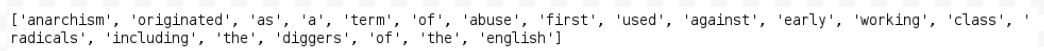
\includegraphics[width=\textwidth]{treshold1}
        \caption{Treshold = $10^{-3}$}
        \label{fig:treshold3}
    \end{subfigure}
   \begin{subfigure}[b]{\textwidth}
        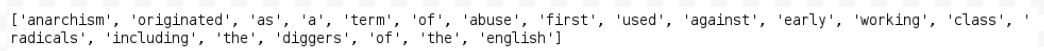
\includegraphics[width=\textwidth]{treshold1}
        \caption{Treshold = $10^{-4}$}
        \label{fig:treshold4}
    \end{subfigure}
     \begin{subfigure}[b]{\textwidth}
        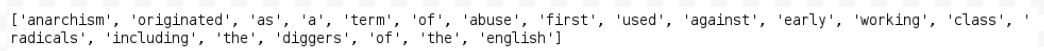
\includegraphics[width=\textwidth]{treshold1}
        \caption{Treshold = $10^{-5}$}
        \label{fig:treshold5}
    \end{subfigure}
    \caption{Example of a sentence with different sampling tresholds}\label{fig:treshold_examples}
\end{figure}

\subsubsection{Min count}
We also applied a threshold in the lower bound, we deleted every word that did not appear more than 5 times in our dataset. We got this tecnique from gensim \cite{gensim}, that introduced this parameter into their training. This is a good technique because of two reasons: first certain words of our data sets do not appear in a common lexicon (twigleg, melqu), or words from a foreign language (gastarbeiter), or names and acronyms. Secondly a word that only appears one time in our dataset will be very dependent on it's original initialization as it will only be updated with it's context pairs. Therefore we applied this technique. It should in theory, such as subsampling, improve the accuracy and  decrease computation time. 

\section{Word similarity}
Evaluating word embedding is not an easy task. We cannot split our data set into train and test set. As the task that the network is learning is of no interest to us. Therefore we need to verify that our embedding are of quality with other techniques. To define quality we first need to define a measure of similarity between two vectors. We will use the cosine distance for this task. The cosine distance of vectors $v$ and $w$ is 1 minus the cosine of the angle between the two vectors. The cosine distance is 0 if two vectors are pointing in the same direction. It's 1 if they are 90 degrees from each other and 2 if they are pointing exactly in the opposite direction. The cosine of the angle between two vectors is calculated by taking the dot product of $v$ and $w$ and dividing it by the magnitude of $v$ and $w$ multiplied with each other. We get then for the cosine distance:
\begin{equation}
cos\_dis(v,w) =1 - \frac{v \cdot w}{|v| |w|} 
\end{equation}

By subtracting 1 from the angle we create a distance between the two vectors, this distance does not take into account any order of magnitude.  Hence for our tasks, two vectors will be considered equal if they are of different magnitude but point in the same direction. 
This technique a part from being shown empirically to work very well to measure the quality of word embedding has another advantage. By normalizing the vectors the calculation of the cosine angle becomes the dot product of the two vectors. Which can be computed very fast on modern gpu's. 

Know that we have a measure to compute the similairty of two vectors let us introduce a way to rate the quality of our embedings.


\subsubsection{wordsim353}
To measure the quality of our word embedding we will need a dataset to compare our results too. We chose  wordsim353\footnote{wordsim353} for this task, as it's the most used in similar literature. The data set consits of 353 pairs of words rated by humans on their similarity. The similarity score is in the range of 1 and 10. See \ref{fig:ws353_ex} for two examples of such pairs. We will rank our embedings on the pearson corelation coefficient between the cosine distance and the scores attributed by humans. 
\begin{figure}[ht]
    \centering
			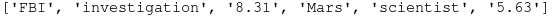
\includegraphics[scale=0.7]{images/wordsim353_example} 
    \caption{Example of pairs and their rating in wordsim353}
    \label{fig:ws353_ex}
\end{figure}

\section{Configuration of the network}
The skip gram model, has a lot of possible options, that can be tuned. We configured one model and then only changed the learning rate. The explanation of the parameters will be structerd as follow: 
\texttt{Parameter} - Description and tuning -  \textit{Value}
\begin{itemize}
\item \texttt{Negative Samples} Here we have to find a trade off between, setting the parameter too high which will result in increased accuracy but a longer computation time. For smaller dataset a higher negative samples is often needed. We experimented early with 5, 10,15 - \textit{10}
\item \texttt{Context Window:} The bigger the window the more training examples the network will have, but if the window is to big the semantic meaning of the window will be erased. Mikolov et al. proposed a setting between 2-10. - \textit{5}
\item\texttt{ Dimension of the embedding}: Here the choice is less obvious, the higher the dimension the better the embedding should be.( cite paper dimension vectors talk about gensim ) but when tested on gensim 100 yielded better results than 300 - \textit{100}
\item \texttt{Batch size}: As described in section FORWARD, there is a trade off to find between accuracy and training time. We first used a batch size of 5000, but then decide after non conclusive results  that 2000 would be better - \textit{2000}
\item \texttt{Alpha}: learnng rate, this hyper parameter was tuned in every optimizer therefore only the range will be indicated - \textit{(1e-5,1)}
\end{itemize}

\section{Input Shuffling}
We used input shuffling as a technique to optimize the skip gram model. We will first describe input shuffling in a general way and then explain why we suppose that input shuffling could work well on the skip gram model. 
Let $X = {x_1...x_n}$ be our input data set. Input Shuffling describes the process of taking a random permutation of the dataset as an input at each epoch. 
The idea behind this technique, is the same as the use of mini batches. We want to present our optimizer with different loss surfaces, so that it's able to find the best optimum. But both combined can be a very powerful, there always lies a risk that a mini-batch isn't a good representative of the true gradient. This way, by shuffling the input, one would avoid this bias.
There are two reasons why we thnik that input shuffling is particulary well suited for the skip gram model. The first one has to do with the fact that when we read our words sequentially that words that only appear very early will not benefit from the context words being already updated from others. The second thing is that we used the special batch technique described in section x.  When using this technique and not using shuffling we will always have words that appear next to each other in a batch and will therefore updat similar words at the same time. We then loose some accuracy. But if instead we would use input shuffling then in one batch the words would likely not be similar and therefore overwriting will be less likely. 
One thing to consider is that when using input shuffling we cannot use a sliding window size. 

\section{Convergence time} 
To optimize convergence time we have to define convergence time first. Therefore we used the already available implementation gensim. we know from \cite{intel}. that a score of $0.66$ in the task of word similarity is the state of the art. We also know after testing Gensim ( more on this process in section discussion), that it takes 4 epochs to converge. Therefore we defined the following criteria for convergence: \\
$\rho - \rho_{prev} < 0.009 \vee or \rho = 0.66$ \\
where $\rho$ is the pearson coefficient with the wordsim353 task. 

\section{Results by optimizer}
We ran multiple experiments for each optimizer. This section will only give an overview over the quantified results. 

\subsection{SGD}
The first challenge for each optimizer was to find a correct learning rate. We first tried the learning rate suggested by gensim, and then performed a random search to find the best one.As expected a bell curve shape resulted, with a learning rate that is to high our model diverged and with a learning rate that is two low or model would not learn quick enough. The best setting that we found is $0.0075$. We converged in 11 epochs. The second experiment was to add input shuffling. 
As seen is figure \ref{fig:results_sgd}, for every learning rate the convergence time decreased. Our model know converges in only 7 epochs. Another intersting point to point out of figure \ref{fig:results_sgd} is that with input shuffling we achieved better results with higher learning rates. As for learning rates of $0.01$ and $0.025$ we did converge in 11 epochs with input shuffling but did not converge in 20 epochs without it.

\begin{figure}[h]
    \centering
			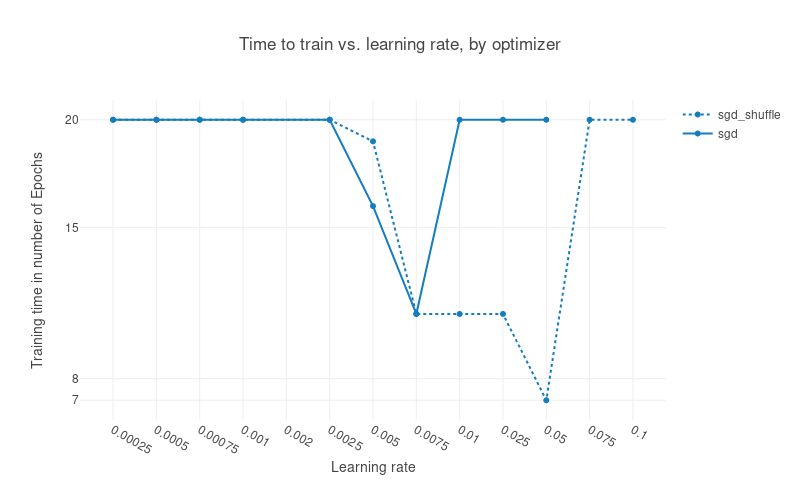
\includegraphics[scale=0.45]{images/results_sgd_shuffle} 
    \caption{Training time Stochastic Gradient Descent with input Shuffling}
    \label{fig:results_sgd}
\end{figure}
\subsection{Momentum and Nesterov}
Momentum and Nesterov accelerated gradient both have an additional hyper parameter $\gamma$, that, as described in Section \ref{optimizers}, defines the percentage of the previous gradient that will be added to the current gradients. We set $\gamma = 0.9$ as this is the typical value, and did not alter it during our experiments. Momentum and Nesterov alone respectively only slightly decrease or increase the convergence time. As the first one optimally converges in 9 epochs and the second one in 13. If we add input shuffling to the equation, interestingly the same things appear as with plain SGD. The convergence time gets better, 8 and 3 epochs until convergence respectively, and higher learning rate do also yield better results. 
\begin{figure}[h]
\centering
\begin{minipage}{.5\textwidth}
  \centering
  	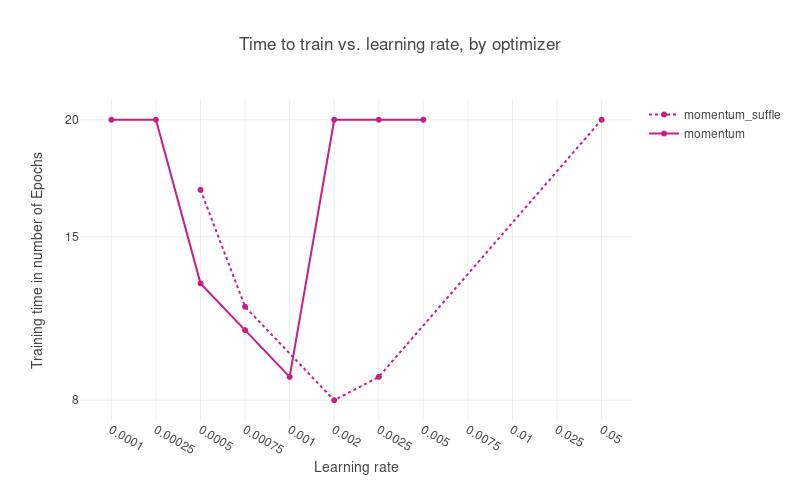
\includegraphics[scale=0.3]{images/results_mom_shuffle} 
    \caption{Training time  Momentum with input Shuffling}
    \label{fig:results_mom}
  \label{fig:test1}
\end{minipage}%
\begin{minipage}{.5\textwidth}
  \centering
	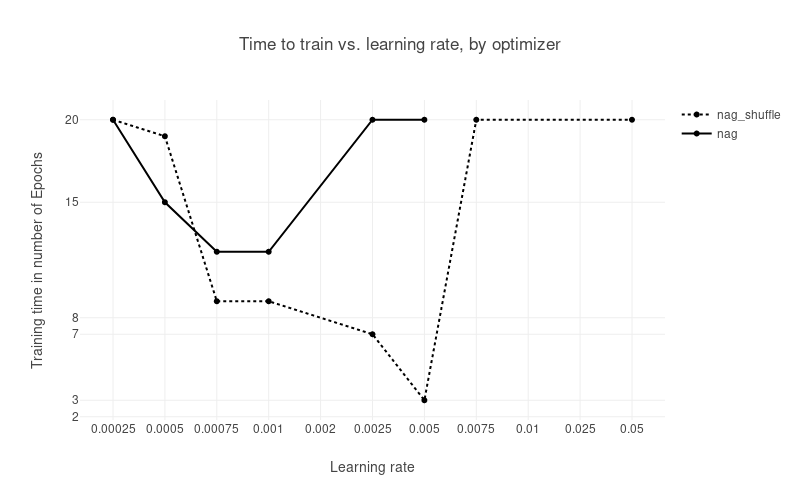
\includegraphics[scale=0.3]{images/results_nag_shuffle} 
    \caption{Training time  Nesterov with input Shuffling}
    \label{fig:results_mom}
\end{minipage}
\end{figure}
\subsection{Adagrad}
Adagrad is a very interesting tool for learning word embedding as they decrease the learning rate for very frequent occuring features, and vice versa for low frequent words. Because words that appear very frequently often do not have a real semantic gain to their context words, it's good to have a low learning rate. So in theory Adagrad is particullary well suited for our task. This was confirmed empirically as our model converged in 4 epochs. When combined with shuffling adagrad only took 3 epochs to converge. This shows the tendency of the skip gram model to converge faster with input shuffling and the big impact of having different learning rate for each feature. 
Here it's interesting to notice that a higher learning rate combined with input shuffling did not yield better results then without shuffling. Both of our best results happened with a learning rate of $0.1$. 
\begin{figure}[h]
    \centering
			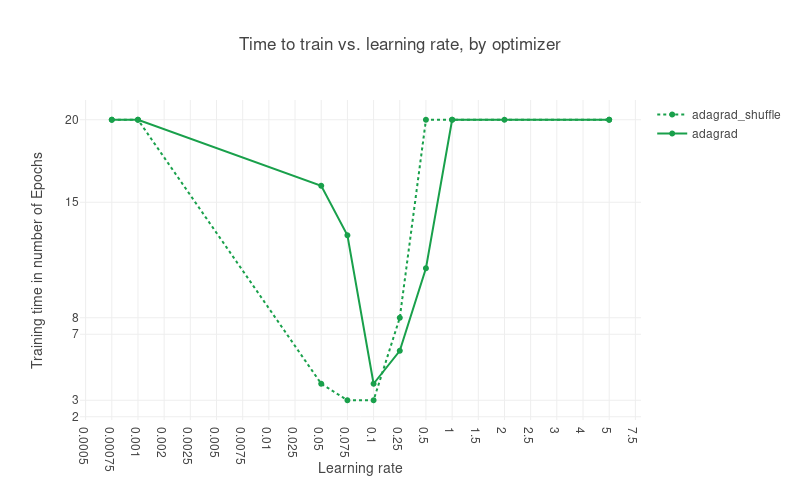
\includegraphics[scale=0.45]{images/results_adagrad_shuffle} 
    \caption{Training time Adagrad with input Shuffling}
    \label{fig:results_adagrad_shuffle}
\end{figure}
\subsection{Adadelta}
In theory Adadelta should outperfrom Adagrad as it's its upgrade. But it did not hold up to our excpectations. Because it didn't has any learning rate to tune, we only did 2 experiments, with and without input shuffling. Adadelta did not manage to achieve a word similarity of 0.66. It only converged to a similarity of 0.59. It did this in 20 epochs without input shuffling and in 3 with input shuffling. As seen in table \ref{table:results_adadelta}
\begin{table}[h]
\centering
\begin{tabular}{|l|l|l|}
\hline
Adadelta Model    & Convergence Time & Word similarity \\ \hline
Without Shuffling & 20               & 0.59            \\ \hline
With Shuffling    & 3                & 0.59            \\ \hline
\end{tabular}
\caption{Convergence Time and Quality with Adadelta}
\label{table:results_adadelta}
\end{table}
\subsection{Adam}
Adam is the most advanced of all the optimizers used in our experiemnts. Did it therefore yield the best results? Indeed this was the case, as seen in figure 2, Adam converged in 3 epochs without shuflfling and 2 with. This are the best result that we got. 
\begin{figure}[h]
    \centering
			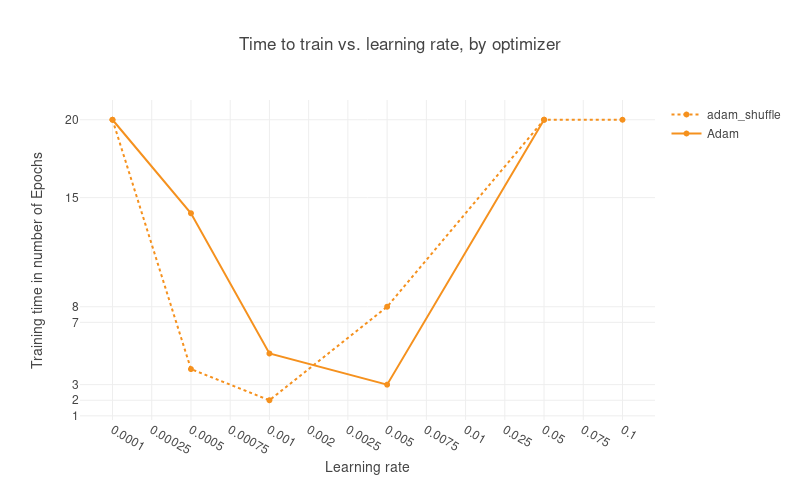
\includegraphics[scale=0.45]{images/results_adam_shuffle} 
    \caption{Training time Adam with input Shuffling}
    \label{fig:results_adam_shuffle}
\end{figure}